%%%%%%%%%%%%%%%%%%%%%%%%%%%%%%%%%%%%%%%%%
% Doctoral Thesis for Faculty of Economics of the University of Porto
%
% %%%%% IMPORTANT %%%%%
% - Requires LuaLaTeX to compile.
% - Bibliography set to use BibLateX and Biber; change the
%   preamble.tex file and the end of this file if you want 
%   to use BibTeX with NatBib.
% %%%%% USAGE INSTRUCTIONS %%%%%
% 1. Edit the MS Word templates for the [covers](<.fep/FEP Capa doutoramento.docx>) (front and back) and the [title page](<.fep/Cover sheet.docx>) (in *portuguese*, *capas* e *folha de rosto*).
% 2. Export the covers as [Front/covers.pdf](Front/covers.pdf) and the title page as [Front/title.pdf](Front/title.pdf).
% 3. Edit the root [vars.tex](vars.tex) file and provide the same info as in the cover and title page when appropriate.
% 4. Review and, eventually, edit [preamble.tex](preamble.tex) file. Don't mess with it if you don't know what to do.
% 5. Edit root [precontent.tex](precontent.tex) file.
% 6. If you want to ensure that all of your labels are being used, check the *Python* script [scripts/check_references.py](scripts/check_references.py) for a way to verify it.
% 7. And, now, edit at will!
%%%%%%%%%%%%%%%%%%%%%%%%%%%%%%%%%%%%%%%%%

% The default font size and two-sided printing
% For a one-sided printing change the flag "twoside" to "oneside"
\documentclass[12pt, twoside]{Thesis}

%-------------------------------------------------------------------------
%   PREAMBLE AND SETTINGS
%-------------------------------------------------------------------------
% Add the preamble. You can change various settings in here
% !TeX root = main.tex
%-------------------------------------------------------------------------
%	PACKAGES AND OTHER DOCUMENT CONFIGURATIONS
%-------------------------------------------------------------------------
% Use Times New Roman as main font
\usepackage{fontspec}
\setmainfont{Times New Roman}

%-------------------------------------------------------------------------
% Table of contents and appendices setup
%-------------------------------------------------------------------------
\usepackage{tocloft}
\tocloftpagestyle{fancy}
\usepackage[toc]{appendix} % 'toc' option includes appendix chapters in ToC
\noappendicestocpagenum % Do not number the appendix page in the ToC

% Alphalph and etoolbox to have Appendix A, B, ..., Z, AA, AB, ... numbering
% https://tex.stackexchange.com/a/134046/289572
\usepackage{alphalph,etoolbox}
\appto\appendix{% patch \appendix so \AlphAlph is used
  \renewcommand\thechapter{\AlphAlph{\value{chapter}}}%
}

% Prevent that the first citation is in the ToC
\usepackage{notoccite}

\setcounter{secnumdepth}{3}
\setcounter{tocdepth}{2}

%-------------------------------------------------------------------------
% Languages setup
%-------------------------------------------------------------------------

% Language hyphenation and typographical rules
\usepackage[portuguese,english]{babel}
\setlocalecaption{english}{bib}{References}
%Custom hyphenization
\hyphenation{Py-thon}
\hyphenation{Ju-py-ter}
\hyphenation{Ma-the-ma-ti-ca}

%-------------------------------------------------------------------------
% Bibliography setup
%-------------------------------------------------------------------------

% Use the natbib reference package - read up on this to edit the reference
% style; if you want text (e.g. Smith et al., 2012) for the in-text references
% (instead of numbers), remove 'numbers'
\usepackage{natbib}
\bibliographystyle{econ}  % Use the econ bibliography style
% If you want to use the 'plain' style, change the above line to:
% \bibliographystyle{plainnat}

% Include pdf pages in the document
% Necessary to include the front pages (cover and etc.)
\usepackage{pdfpages}

% Inline quotes
% added for \begin{displayquote}
\usepackage[autostyle]{csquotes}

% Interesting float placements (like 'H') and custom float types
\usepackage{float}
% Text wrapped around pictures
% https://pt.sharelatex.com/learn/Wrapping_text_around_figures
\usepackage{wrapfig}
% Force float barriers, use as \FloatBarrier
\usepackage[section]{placeins}
% Place floats *above* footnotes
\usepackage[bottom,hang,flushmargin]{footmisc}
% Set default float placement
\makeatletter
\renewcommand{\fps@figure}{tbph}
\renewcommand{\fps@table}{tbph}
\makeatother

% Pretty colours
\usepackage{xcolor}

% SVGs with Inkscape and PDF+LaTeX
% https://tex.stackexchange.com/questions/473994/svg-and-inkscape
\usepackage[inkscapearea=page]{svg}
% Specifies the directory where vector are stored
\svgpath{{Svgs/}}

% Graphics stuff
\usepackage{graphicx}  % invoked by svg
% Specifies the directory where pictures are stored
\graphicspath{{Figures/}}

% For sub-figures and stuff
\usepackage{caption}
\usepackage{subcaption}

%-------------------------------------------------------------------------
% Math stuff setup
%-------------------------------------------------------------------------
\usepackage{amsmath} % Interesting environments
\usepackage{amssymb} % Interesting symbols
\usepackage{commath} % Interesting macros
\usepackage{braket} % Dirac bra-ket and set notations
\usepackage{mathtools} % Mathematical tools to use with amsmath

% Math alphabet
\DeclareMathAlphabet{\pazocal}{OMS}{zplm}{m}{n}
\newcommand{\Sa}{\pazocal{S}}
\newcommand{\Ua}{\pazocal{U}}
\newcommand{\Ha}{\pazocal{H}}
\newcommand{\Fa}{\pazocal{F}}
\newcommand{\Ia}{\pazocal{I}}
\newcommand{\Ea}{\pazocal{E}}
\newcommand{\ja}{\pazocal{J}}

%Custom math operators
\DeclareMathOperator*{\meshgrid}{meshgrid}

% Floor and ceiling of numbers
\DeclarePairedDelimiter\ceil{\lceil}{\rceil}
\DeclarePairedDelimiter\floor{\lfloor}{\rfloor}

% Notation variables
\newcommand{\dd}{\mathrm{d}}

% Units and numbers in text
\usepackage{siunitx}
\DeclareSIUnit\baud{Bd} % Baud

% Reimplementation of and extensions to LaTeX verbatim
\usepackage{verbatim} %added for \begin{comment}

% Fancy chapter start quotes
\usepackage{epigraph, varwidth}
% Overload epigraph command
\renewcommand{\epigraphsize}{\small}
\setlength{\epigraphwidth}{0.90\textwidth}
\renewcommand{\textflush}{flushright}
\renewcommand{\sourceflush}{flushright}
% A useful addition
\newcommand{\epitextfont}{\itshape}
\newcommand{\episourcefont}{\scshape}
\makeatletter
\newsavebox{\epi@textbox}
\newsavebox{\epi@sourcebox}
\newlength\epi@finalwidth
\renewcommand{\epigraph}[2]{%
  \vspace{\beforeepigraphskip}
  {\epigraphsize\begin{\epigraphflush}
   \epi@finalwidth=\z@
   \sbox\epi@textbox{%
     \varwidth{\epigraphwidth}
     \begin{\textflush}\epitextfont#1\end{\textflush}
     \endvarwidth
   }%
   \epi@finalwidth=\wd\epi@textbox
   \sbox\epi@sourcebox{%
     \varwidth{\epigraphwidth}
     \begin{\sourceflush}\episourcefont#2\end{\sourceflush}%
     \endvarwidth
   }%
   \ifdim\wd\epi@sourcebox>\epi@finalwidth
     \epi@finalwidth=\wd\epi@sourcebox
   \fi
   \leavevmode\vbox{
     \hb@xt@\epi@finalwidth{\hfil\box\epi@textbox}
     \vskip1.75ex
     \hrule height \epigraphrule
     \vskip.75ex
     \hb@xt@\epi@finalwidth{\hfil\box\epi@sourcebox}
   }%
   \end{\epigraphflush}
   \vspace{\afterepigraphskip}}}
\makeatother
%End of overload command


% Use more than one optional parameter in a new commands
\usepackage{xargs}

% Hyperref and Backref
% backref makes the bibliography say where the entry was cited.
% For the print version of the thesis you might wanna set all colors to back
\usepackage{hyperref}
\usepackage[hyperpageref]{backref}
\hypersetup{colorlinks, citecolor=black, urlcolor=black,
        linkcolor=black, breaklinks=true, hypertexnames=true}
\renewcommand*{\backref}[1]{}
\renewcommand*{\backrefalt}[4]{%
    \ifcase #1%
          \or [Cited on page~#2.]%
          \else [Cited on pages~#2.]%
    \fi%
    }
% Interesting URL breakings
\usepackage{url}
\def\UrlBreaks{\do\/\do-\do\&\do.\do:}

% Variants of \fbox and other games with boxes
\usepackage{fancybox}

% LaTeX default text is fully-justified, but often left-justified text may be a
% more suitable format. This left-alignment can be easily accomplished by
% importing the ragged2e package.
\usepackage{ragged2e}

% Create tabular cells spanning multiple rows
\usepackage{multirow}
\usepackage{longtable} % For long tables that span multiple pages

% Changes bullet points marker
\renewcommand{\labelitemi}{\(\bullet\)}

% Notes on the documents
% https://tex.stackexchange.com/questions/9796/how-to-add-todo-notes
% https://tex.stackexchange.com/questions/316220/todo-commentsnot-include-and-left-align
% Examples:
% \unsure{Is this correct?}, \change{Change this!},
% \info{This can help me in chapter seven!}
% \improvement{This really needs to be improved!\\ What was I thinking?!}
% \thiswillnotshow{This is hidden since option `disable' is chosen!}
% WARNING: It eliminates whitespaces in front of it.
% You can add trailing {} to avoid.

\usepackage[colorinlistoftodos,
    prependcaption,
    textsize=tiny,
    textwidth=2cm]
        {todonotes}
% You can add:
% \setlength{\marginparwidth}{3cm}\reversemarginpar
% before \todo on each command for a different effect
\newcommandx{\unsure}[2][1=]{
    % \setlength{\marginparwidth}{3cm}\reversemarginpar
    \todo[linecolor=red,backgroundcolor=red!25,bordercolor=red,#1]{#2}
    }
\newcommandx{\change}[2][1=]{
    % \setlength{\marginparwidth}{3cm}\reversemarginpar
    \todo[linecolor=blue,backgroundcolor=blue!25,bordercolor=blue,#1]{#2}
    }
\newcommandx{\info}[2][1=]{
    % \setlength{\marginparwidth}{3cm}\reversemarginpar
    \todo[linecolor=green,backgroundcolor=green!25,bordercolor=green,#1]{#2}
    }
\newcommandx{\improvement}[2][1=]{
    % \setlength{\marginparwidth}{3cm}\reversemarginpar
    \todo[linecolor=yellow,backgroundcolor=yellow!25,bordercolor=yellow,#1]{#2}
    }
\newcommandx{\thiswillnotshow}[2][1=]{\todo[disable,#1]{#2}}


% \usepackage[acronym,toc,shortcuts]{glossaries}
% \makeglossaries
\usepackage{acronym} 

\usepackage{caption}
\captionsetup{justification=raggedright,singlelinecheck=false}

%-------------------------------------------------------------------------
%	Divisions' title formatting
%-------------------------------------------------------------------------
\titleformat{\subsubsection}{\fontsize{12}{0}\selectfont\bfseries}{\thesubsubsection{.}}{1em}{}
\titleformat{\subsection}{\fontsize{12}{0}\selectfont\bfseries}{\thesubsection{.}}{1em}{}
\titleformat{\section}{\fontsize{14}{0}\selectfont\bfseries}{\thesection{.}}{1em}{}
\titleformat{\chapter}[hang]{\fontsize{20}{0}\selectfont\bfseries}{\thechapter{.}}{1em}{}

\titlespacing\chapter{0pt}{12pt plus 4pt minus 2pt}{0pt plus 2pt minus 2pt}
\titlespacing\section{0pt}{12pt plus 4pt minus 2pt}{0pt plus 2pt minus 2pt}
\titlespacing\subsection{0pt}{12pt plus 4pt minus 2pt}{0pt plus 2pt minus 2pt}
\titlespacing\subsubsection{0pt}{12pt plus 4pt minus 2pt}{0pt plus 2pt minus 2pt}

% Python and MATLAB styles for code blocks
\usepackage{pythonhighlight}
\usepackage{matlab-prettifier}

% Thesis settings. THIS IS VERY IMPORTANT YOU CHANGE
% !TEX root = main.tex

%-------------------------------------------------------------------------
%	PARAMETERS FOR FCUP THESIS TITLEPAGES/BOOK COVER
%-------------------------------------------------------------------------

% THESIS TYPEs:
% - msc (Master of Sciences)
% - phd (Doctor of Philosophy)
\thesistype{msc}

% Book spine width (CAREFUL: MIN 8mm)
\spinewidth{10mm}

% Thesis front title
\fronttitle{My Thesis Title}

% Front title spacing multiplier
% NOTE: you may want to adjust this value to 1.15/1.20 after changing to your
% thesis title
\titlespacing{1.15}

% Book spine title
\spinetitle{Spine Title}

% Author name
\authorname[mailto:example@fc.up.pt]{John Smith}

% Affiliation number 2
% USAGE: \otheraffiliation[url]{relative/path/to/logo}{INITIAL}{University name}
%\otheraffiliation[http://uni2.pt]{logos/logo2}{UNI2}{Universidade/Faculdade 2}

% Affiliation number 3
% USAGE: \extraaffiliation[url]{relative/path/to/logo}{INITIAL}{University name}
%\extraaffiliation[http://uni3.pt]{logos/logo3}{UNI3}{Universidade/Faculdade 3}

% Degree name
\degreename{Mestrado Integrado em Engenharia Física}

% Field of science
\sciencefield{Engenharia Física}

% Department name
\department[http://dfa.fc.up.pt/]{Departamento de Física e Astronomia}

% Supervisor info
% Supervisor name
\supervisor[mailto:example@fc.up.pt]{Prof. Dra. Marie Curie}
% Supervisor name position/Category (comment out to hide this field)
%\supervisorposition{Categoria} %
% Supervisor university/faculty
\supervisoraffiliation[]{Faculdade de Ciências}
% Supervisor secondary affiliation
%\supervisoraffiliation[]{Instituto de Engenharia de Sistemas e Computadores,
% Tecnologia e Ciência}

% Cosupervisor info ----- Comment out if not needed
% Cosupervisor name
\cosupervisor[mailto:example@fc.up.pt]{Prof. Dr. Galileu Galilei}
% Cosupervisor name position/Category (comment out to hide this field)
%\cosupervisorposition{Categoria}
% Supervisor university/faculty
\cosupervisoraffiliation[]{Faculdade de Ciências}

% ------------------

%-------------------------------------------------------------------------
%	DOCUMENT
%-------------------------------------------------------------------------
\begin{document}

% Start counting pages in an unused scheme to fix backref
\pagenumbering{Alph}

% Includes the front pages (cover and etc.)
\pagestyle{empty}

\includepdf[pages={1},pagecommand={},scale=1]{Front/covers}
\cleardoublepage

\includepdf[pages={1},pagecommand={},scale=1]{Front/title}
\cleardoublepage
\pagestyle{fancy}

%-------------------------------------------------------------------------

% Use roman page numbering style (i, ii, iii, iv...) for the pre-content pages
\frontmatter

% Edit this file!

%-------------------------------------------------------------------------
%	QUOTATION PAGE
%-------------------------------------------------------------------------
%\quotepage{Matt Smith as \emph{The Doctor}, written by Matthew Graham}
%{
%	I am and always will be the optimist, the hoper of far-flung hopes and the
%	dreamer of \newline improbable dreams
%}

%-------------------------------------------------------------------------
%	DEDICATORY
%-------------------------------------------------------------------------

%\begin{dedicatory}
%	Dedicated to (optional) 
%\end{dedicatory}

%-------------------------------------------------------------------------
%	ACKNOWLEDGEMENTS PAGE
%-------------------------------------------------------------------------
\addtocontents{toc}{\protect\setcounter{tocdepth}{-1}}
\begin{acknowledgements}

Acknowledge ALL the people!

\end{acknowledgements}
\addtocontents{toc}{\protect\setcounter{tocdepth}{3}}
%\addvspacetoc{0.3cm} % Add a gap in the Contents, for aesthetics


%-------------------------------------------------------------------------
%	ABSTRACT PAGE (PORTUGUESE)
%-------------------------------------------------------------------------
\addtocontents{toc}{\protect\setcounter{tocdepth}{-1}}
\begin{abstract}[
	thesistitle={Titulo da Tese em Portugês},
	title={Resumo},
	degree={Mestrado Integrado em Engenharia Física},
	nameconnector={por},
        keywordsname={Palavras-chave},
        keywords={física (keywords em português)}]
\begin{otherlanguage}{portuguese}

Este tese é sobre alguma coisa



\end{otherlanguage}
\end{abstract}
\addtocontents{toc}{\protect\setcounter{tocdepth}{3}}
%-------------------------------------------------------------------------
%	ABSTRACT PAGE
%-------------------------------------------------------------------------
\addtocontents{toc}{\protect\setcounter{tocdepth}{-1}}
\begin{abstract}

This thesis is about something, I guess.

\end{abstract}
\addtocontents{toc}{\protect\setcounter{tocdepth}{3}}

%-------------------------------------------------------------------------
%	LIST OF CONTENTS/FIGURES/TABLES
%-------------------------------------------------------------------------

\addtocontents{toc}{\protect\setcounter{tocdepth}{-1}}

\tableofcontents % Write out the Table of Contents

\addtocontents{toc}{\protect\setcounter{tocdepth}{3}}
\addvspacetoc{0.3cm}

%\listoftables % Write out the List of Tables

\listoffigures % Write out the List of Figures



%\addvspacetoc{0.3cm}

%-------------------------------------------------------------------------
%	PHYSICAL CONSTANTS/OTHER DEFINITIONS
%-------------------------------------------------------------------------

%\begin{listofcontants}
%	\const{My little ponny test of magical rainbow}{$mn/mp$}
%    {$2.997\ 924\ 58\times10^{8}\ \mbox{ms}^{-\mbox{s}}$}
%   \const{Vaccuum permeability test of magical rainbow for a specific case of
%   condensed matter physics}
%   {$\epsilon_0$}{$2.997\ 924\ 58\times10^{8}\ \mbox{ms}^{-\mbox{s}}$}
%	\const{Speed of Light test of magical rainbow}{$c$}
%    {$2.997\ 924\ 58\times10^{8}\ \mbox{ms}^{-\mbox{s}}$}
%\end{listofcontants}


%-------------------------------------------------------------------------
%	SYMBOLS
%-------------------------------------------------------------------------

%\begin{listofsymbols}
%	\symb{$F_{\mu\nu}$}{Maxwell tensor}{F}
%	\symb{$a$}{distance}{m}
%	\\
%	\symb{$\omega$}{angular frequency}{rads$^{-1}$}
%\end{listofsymbols}


%-------------------------------------------------------------------------
%	NOTATION
%-------------------------------------------------------------------------

% \newcommand\notationname{Notation and Conventions}
% \addtotoc{\notationname}
% \fancyhead[LO]{\textsc{\notationname}}

% \input{Notation}



%-------------------------------------------------------------------------
%	ABBREVIATIONS
%-------------------------------------------------------------------------

\newacronym{ann}{ANN}{Artificial Neural Network}

\printglossary[type=\acronymtype,title={List of Abbreviations}]


%-------------------------------------------------------------------------
%	THESIS CONTENT - CHAPTERS
%-------------------------------------------------------------------------

% Begin numeric (1,2,3...) page numbering
\mainmatter

\pagestyle{fancy}
\renewcommand{\chaptermark}[1]{\markboth{\thechapter. \textsc{#1}}{}}
%\fancyhead[LO]{\leftmark}

%%% -----------  ADD CHAPTERS HERE ------------------ %%%
% Chapter Template

% Main chapter title
%\chapter[toc version]{doc version}
\chapter{Chapter Title Here}

% Short version of the title for the header
%\chaptermark{version for header}

% Chapter Label
% For referencing this chapter elsewhere, use \ref{ChapterTemplate}
\label{ChapterTemplate}

% Write text in here
% Use \subsection and \subsubsection to organize text

This is a thesis model for the FEP PhD thesis. It's an attempt to adapt the 
\href{https://www.overleaf.com/latex/templates/fcup-thesis-layout-2024/gpbvtwzckzgm}{FCUP thesis layout 2024}, 
available at \href{https://www.overleaf.com/}{Overleaf}, 
to the August 2025 \href{https://sigarra.up.pt/fep/pt/conteudos_geral.ver?pct_pag_id=1009493\&pct_parametros=pv_unidade=7\&pct_grupo=28581\#28581}{FEP's rules for PhD thesis}.

Welcome to the tutorial on how to use this thesis model. This is not to teach
you how to use \LaTeX. For that read a tutorial. But this aims to teach you how
to do the basic stuff you will need in order to produce a decent document.
We can start with a section and a section epigraph:

\section{Citations}
\epigraph{Python is a truly wonderful language. When somebody comes up with a good idea it takes about 1 minute and five lines to program something that almost does what you want. Then it takes only an hour to extend the script to 300 lines, after which it still does almost what you want.}{Dr. Jack Jansen,  maintainer of MacPython}

You can add extra info to you references, like~\parencite[section 3]{Fienup1982}. You
can also call them by author, like saying~\textcite{Fienup1982}\unsure{You can make
personal notes like this}.

Also a random displayquote thing:

\begin{displayquote}
    How can we image an object that's behind or enclosed on a medium where light does not propagate trivially? How can we manipulate light propagating in these media?
\end{displayquote}

Lean manufacturing has been a transformative approach in industrial operations, 
particularly in the UK, where its early adoption was documented by \textcite{voss1987jit}. 
The theoretical underpinnings of investment decisions under asymmetric information, 
which are crucial to understanding capital allocation in such environments, 
were explored by \textcite{daniel1995financing} in a comprehensive handbook on finance. 
Broader historical context is provided by \textcite{womack1990machine}, who trace 
the evolution of lean production and its global impact. In the Portuguese context, 
structural economic challenges and their implications for development were 
analyzed by \textcite{goncalves1995problemas}, offering insights into national 
policy constraints. More recently, the integration of lightweight formal methods into 
recruitment engineering has been being discussed in the literature. Some works 
highlight the role of digital tools in modern organizational processes \parencite[e.g.,][]{george2003application}.

\section{Figures}

Let us start with a figure with two subfigures like in~\ref{fig:FCUPfatCat}.
\begin{figure}
	\centering
	\begin{subfigure}{.49\textwidth}
  		\centering
          
\includegraphics[width=.95\linewidth]
            {ChapterTemplate/20160517_123603.jpg}
  		\caption{FCUP's fat cat doing what cats do.}
	\end{subfigure}%
	\hfill
	\begin{subfigure}{.49\textwidth}
  		\centering
          
\includegraphics[width=.95\linewidth]
            {ChapterTemplate/20160517_123609.jpg}
 		 \caption{FCUP's fat cat resting.}
	\end{subfigure}
	\caption{\label{fig:FCUPfatCat}FCUP's fat cat.}
\end{figure}


Or two figures side by side like~\ref{fig:FCUPfatcatSide1}
and~\ref{fig:FCUPfatcatSide2}.

\begin{figure}
\centering
\begin{minipage}{.49\textwidth}
  \centering
  
\includegraphics[width=.95\linewidth]{ChapterTemplate/20160517_123603.jpg}
  \captionof{figure}{\label{fig:FCUPfatcatSide1}FCUP's fat cat doing what cats do.}
\end{minipage}%
\hfill
\begin{minipage}{.49\textwidth}
  \centering
  
\includegraphics[width=.95\linewidth]{ChapterTemplate/20160517_123609.jpg}
  \captionof{figure}{\label{fig:FCUPfatcatSide2}FCUP's fat cat.}
\end{minipage}
\end{figure}


Or a figure with some text on the side, like~\ref{fig:FCUPfatcatSide3}, or even
a figure wrapped around in text, as seen on Figure~\ref{fig:FCUPfatcatSide4}.

\begin{figure}
\centering
\begin{minipage}{.49\textwidth}
  And here we have some text related to this image. The text can occupy the same space as the image would normally do.
\end{minipage}%
\hfill
\begin{minipage}{.49\textwidth}
  \centering
  
\includegraphics[width=.95\linewidth]{ChapterTemplate/20160517_123609.jpg}
  \captionof{figure}{\label{fig:FCUPfatcatSide3}FCUP's fat cat.}
\end{minipage}
\end{figure}

\textcolor{red}{This is where the float goes with text wrapping around it. You
may embed tabular environment inside wraptable environment and customize as you
like:} Ultrices dui sapien eget mi proin sed libero. Ornare lectus sit amet est
placerat in egestas erat imperdiet. Tortor dignissim convallis aenean et. Quam
adipiscing vitae proin sagittis nisl rhoncus mattis. Vivamus at augue eget arcu
dictum varius duis. Cursus turpis massa tincidunt dui.
\begin{wrapfigure}{r}{8cm}
    % If you find figures split between two pages, use the uppercase L or R, to
    % let the wrapped figure be a float object that can move through the page.
    \centering
    
\includegraphics[width=7cm]{ChapterTemplate/20160517_123609.jpg}
    \captionof{figure}{\label{fig:FCUPfatcatSide4}FCUP's fat cat.}
  \end{wrapfigure}
Leo in vitae turpis massa sed. Tempor orci eu lobortis elementum. Turpis egestas
integer eget aliquet nibh praesent tristique magna. Sed blandit libero volutpat
sed cras ornare arcu dui. Feugiat sed lectus vestibulum mattis ullamcorper velit
sed ullamcorper. Interdum velit euismod in pellentesque massa placerat duis
ultricies lacus. Ac ut consequat semper viverra nam. Dis parturient montes
nascetur ridiculus mus. Mattis pellentesque id nibh tortor.

\subsection{SVGs}
How to make a \LaTeX\ document with vector images, where the text in the images
has exactly the same font and size as in normal text? This article describes how
this is done using the `PDF/EPS/PS + LaTeX' output feature of Inkscape 0.48.
Inkscape can export the graphics to PDF/EPS/PS, and the text to a \LaTeX\ file.
When the \LaTeX\ file is input in the \LaTeX\ document, the PDF/EPS/PS image is
included with overlaid text. Because typesetting of the text is done by \LaTeX,
\LaTeX\ commands can be used in images, such as writing equations, references
and shorthand macros.

\emph{(requires Inkscape version 0.48 or higher; this document discusses features up to Inkscape 0.49)}

\begin{figure}
    \centering
      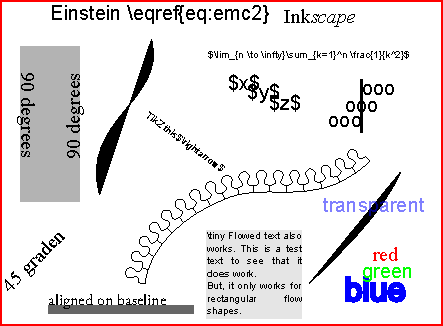
\includegraphics[width=0.5\columnwidth]{ChapterTemplate/image-normal.pdf}
      \caption[The test SVG image, as it is seen in Inkscape]
      {The test SVG image, as it is seen in Inkscape (exported to PDF
      \emph{without} \LaTeX\ option).}
      \label{fig:normal}
\end{figure}

\begin{figure}
\centering
    \includesvg[width=0.8\columnwidth]{image}
    \caption{The test image, exported to PDF \emph{with} \LaTeX\ option.}
    \label{fig:pdflatex}
\end{figure}

\begin{equation}
    \label{eq:emc2}
    E = mc^{2}
\end{equation}

\subsubsection{Automatic export}

(`write18' must be enabled, see the {\small\verb|epstopdf|} package
documentation. Add {\small\verb|-shell-escape|} to the command line when calling
{\small\verb|pdflatex|}. \textcolor{red}{And inkscape must be discoverable by the
OS}),

Whenever the SVG file is updated, it is possible to have \LaTeX\ automatically call Inkscape to export the image to PDF and \LaTeX\ again. This simplifies the workflow to
\begin{itemize}
	\item Modify the SVG image in Inkscape;
	\item Save the SVG (Ctrl+S, no need to export to PDF);
	\item Recompile \LaTeX\ document. pdf\LaTeX\ will notice the SVG file has changed, and will automatically do the export for you.
\end{itemize}

\section{Math}

The following equation uses a custom mathematical operator defined in line 88
of preamble.tex:
\begin{equation}
\begin{aligned}
            \meshgrid_{\mathbf{x}_{1},\mathbf{x}_{2}}\mathbf{x}_{1}&=
            \begin{bmatrix}a_{1} & b_{1} & c_{1}\\
            a_{1} & b_{1} & c_{1}
\end{bmatrix}\\
            \meshgrid_{\mathbf{x}_{1},\mathbf{x}_{2}}\mathbf{x}_{2}&=
            \begin{bmatrix}a_{2} & a_{2} & a_{2}\\
            b_{2} & b_{2} & b_{2}
\end{bmatrix}
\end{aligned}
\end{equation}

The following equation uses the custom ceil and floor operator defined in line 86 of the stock preamble.tex:

\begin{equation}
x = \floor*{\frac{y}{2}} + \ceil*{\frac{w}{2}}
\end{equation}


And this is an equation with multiple lines:
\begin{equation}
\begin{aligned}
&I_{0}=I^{\prime}+I^{\prime\prime}\cos(\varPsi)   \\
&I_{\pi/2}=-I^{\prime\prime}\sin(\varPsi)                \\
&I_{\pi}=I^{\prime}-I^{\prime\prime}\cos(\varPsi)   \\
&I_{3\pi/2}=I^{\prime\prime}\sin(\varPsi)
\end{aligned}
\end{equation}

This is some MATLAB code:
\begin{lstlisting}[style=Matlab-editor]
% Sample MATLAB Code: Plotting a Sine Wave

% Define the time vector from 0 to 2*pi with small increments
t = 0:0.01:2*pi;

% Compute the sine of each time point
y = sin(t);

% Create the plot
figure;
plot(t, y, 'b-', 'LineWidth', 2);

% Add title and labels
title('Sine Wave');
xlabel('Time (radians)');
ylabel('Amplitude');

% Add grid
grid on;
\end{lstlisting}

And this is some random Python code:

\begin{python}
def Hello():
    """
      Meaningful docstring with in-depth explanation of this function
    """
    print(``Hello World !!'')

if __name__ == '__main__':
    Hello()
\end{python}

\section{Abreviations}

\begin{acronym}
    \acro{ann}{artificial neural network}
\end{acronym}

Use acronyms like this: \ac{ann}

\section{Fonts}

The main document font is \fontname\font, line spacing \the\baselineskip.\footnote{Footnote font is: \fontname\font
. Line spacing was left at its default value in footnotes: \the\baselineskip}.

\section{Tables}

Table~\ref{table:data} shows how to add a table caption and reference a table.
\begin{table}[h!]
\centering
\begin{tabular}{||c c c c||} 
 \hline
 Col1 & Col2 & Col2 & Col3 \\ [0.5ex] 
 \hline\hline
 1 & 6 & 87837 & 787 \\ 
 2 & 7 & 78 & 5415 \\
 3 & 545 & 778 & 7507 \\
 4 & 545 & 18744 & 7560 \\
 5 & 88 & 788 & 6344 \\ [1ex] 
 \hline
\end{tabular}
\caption{Table to test captions and labels.}
\label{table:data}
\end{table}

Table~\ref{tab:longexample} that follows is an example of a long table.
\begin{center}
\begin{longtable}{|p{0.07\textwidth}|p{0.15\textwidth}|p{0.6\textwidth}|}
\caption{My Long Table Example} \label{tab:longexample} \\
\hline
\textbf{ID} & \textbf{Name} & \textbf{Description} \\
\hline
\endfirsthead

\hline
\textbf{ID} & \textbf{Name} & \textbf{Description} \\
\hline
\endhead

\hline
\endfoot

\hline
\endlastfoot

1 & Alice & Loremipsumdolor sit amet, consectetuer adipi
scing elit. Ut purus elit, vestibulumut, place
rat ac, adipiscingvitae, felis. Curabiturdictum
 gravidamauris.Namarculibero,nonummyeget,
 consectetuer id,vulputatea,magna. Donecvehi
culaaugueeuneque.Pellentesquehabitantmorbi
 tristiquesenectusetnetusetmalesuadafamesac
 turpis egestas. Maurisut leo. Crasviverrame
tusrhoncussem.Nullaet lectusvestibulumurna
 fringillaultrices. Phaselluseutellussitamettor
torgravidaplacerat. Integersapienest, iaculisin,
 pretiumquis,viverraac,nunc.Praesentegetsem
 velleoultricesbibendum.Aeneanfaucibus.Morbi
 dolornulla,malesuadaeu,pulvinarat,mollisac,
 nulla. Curabiturauctorsempernulla. Donecva
riusorciegetrisus.Duisnibhmi,congueeu,accu
msaneleifend, sagittisquis,diam. Duisegetorci
 sitametorcidignissimrutrum. \\
2 & Bob & Namdui ligula, fringillaa, euismodsodales, sol
licitudinvel,wisi.Morbiauctor loremnonjusto.
 Namlacuslibero,pretiumat, lobortisvitae,ultri
cieset,tellus.Donecaliquet,tortorsedaccumsan
 bibendum,eratligulaaliquetmagna,vitaeornare
 odiometusami. Morbi acorci etnislhendrerit
 mollis. Suspendisseutmassa.Crasnecante.Pel
lentesqueanulla. Cumsociisnatoquepenatibus
 etmagnisdisparturientmontes,nascetur ridicu
lusmus.Aliquamtincidunturna.Nullaullamcor
pervestibulumturpis. Pellentesquecursus luctus
 mauris. \\
3 & Carol & Nullamalesuadaporttitordiam.Donecfeliserat,
 congue non, volutpat at, tincidunt tristique, li
bero. Vivamus viverra fermentumfelis. Donec
 nonummypellentesqueante. Phasellusadipiscing
 semperelit.Proinfermentummassaacquam.Sed
 diamturpis,molestievitae, placerat a,molestie
 nec,leo.Maecenaslacinia.Namipsumligula,elei
fendat, accumsannec, suscipita, ipsum. Morbi
 blandit ligula feugiatmagna. Nunceleifendcon
sequat lorem. Sed lacinianullavitaeenim. Pel
lentesquetinciduntpurusvelmagna. Integernon
 enim. Praesent euismodnunc eupurus. Donec
 bibendumquamintellus. Nullamcursuspulvi
narlectus.Donecetmi.Namvulputatemetuseu
 enim.Vestibulumpellentesquefeliseumassa. \\
4 & Dave & Quisqueullamcorperplacerat ipsum. Crasnibh.
 Morbivel justovitaelacustinciduntultrices. Lo
remipsumdolorsitamet,consectetueradipiscing
 elit. Inhachabitasseplateadictumst. Integer
 tempusconvallisaugue.Etiamfacilisis.Nuncele
mentumfermentumwisi. Aeneanplacerat. Ut
 imperdiet,enimsedgravidasollicitudin, felisodio
 placeratquam, acpulvinar elitpurus eget enim.
 Nuncvitae tortor. Proin tempus nibh sit amet
 nisl. Vivamusquis tortorvitae risusportavehi
cula. \\
% Add more rows as needed
\end{longtable}

Finally, Table~\ref{tab:scores} is a  three-part table with notes.

\begin{threeparttable}
\caption{Student scores by department.} \label{tab:scores}
\begin{tabular}{llr}
\toprule
\textbf{Name} & \textbf{Department} & \textbf{Score} \\
\midrule
Alice\tnote{1} & Physics & 95 \\
Bob\tnote{2} & Mathematics & 89 \\
Carol & Chemistry & 92 \\
\bottomrule
\end{tabular}
\begin{tablenotes}
\item \textbf{Note:} Main note of the table.
\small
\item[1] Alice received extra credit.
\item[2] Bob's score includes a project bonus.
\end{tablenotes}
\end{threeparttable}
\end{center}
% Add others as needed

%-------------------------------------------------------------------------
%	THESIS CONTENT - APPENDICES
%-------------------------------------------------------------------------
\appendix % Cue to tell LaTeX that the following 'chapters' are Appendices
\cleardoublepage
\appendixpage

%%% -----------  ADD APPENDIX HERE ------------------ %%%
% Appendix Template

\chapter*{Appendix Title Here} % Main appendix title

\label{AppendixX} % Change X to a consecutive letter; for referencing this appendix elsewhere, use \ref{AppendixX}

Write your Appendix content here.
%\input{Appendices/AppendixB}
%\input{Appendices/AppendixC}

\backmatter

%-------------------------------------------------------------------------
%	BIBLIOGRAPHY
%-------------------------------------------------------------------------
\printbibliography[heading=bibintoc]
% for bibtex:
% \phantomsection
% \addcontentsline{toc}{chapter}{References}
%  % The references are stored in the file "Bibliography.bib"
% \bibliography{Bibliography}

%-------------------------------------------------------------------------
%	BACK COVER
%-------------------------------------------------------------------------
\cleardoublepage
\hbox{}
\thispagestyle{empty}

% adds the blank pages before the back cover
\cleardoublepage
\hbox{}
\thispagestyle{empty}

% Include the back cover
\newpage
\thispagestyle{empty}

\includepdf[pages={2},pagecommand={},scale=1]{Front/covers}

\end{document}